% main.tex
\documentclass{layout}

\titulo{Compensador por Avanço}
\autor{William Sleman}
\materia{Sistemas de Controle II}
\mes_ano{09/2023}
\professor{Douglas Haupt}



\begin{document}

\printtitle

\noindent \textbf{1)} Projetar um compensador por avanço de fase para a planta cuja função de transferência, $G(s)$, é:
\[ G(s) = \dfrac{4}{s\cdot (s+2)}\]

\color{Red}
\noindent \textbf{Solução:}


\color{Black}
Para o projeto foi utilizado o Matlab, com o seguinte código:

\lstinputlisting[style=Matlab]{Compensador_por_avanco.m}

\noindent \textbf{Images Output:}

\begin{figure}[H]
    \centering
    \begin{subfigure}[b]{0.49\textwidth}
        \centering
        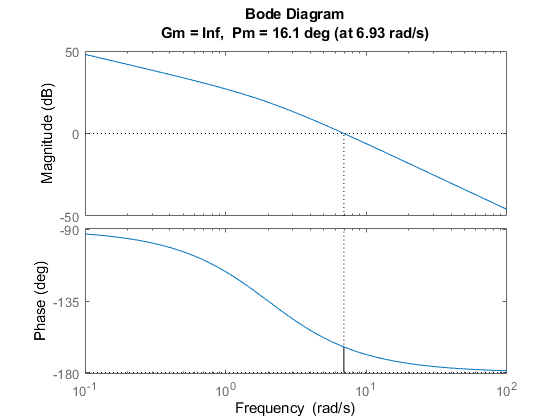
\includegraphics[width=\textwidth]{images/figure1.png}
    \end{subfigure}
    \hfill
    \begin{subfigure}[b]{0.49\textwidth}
        \centering
        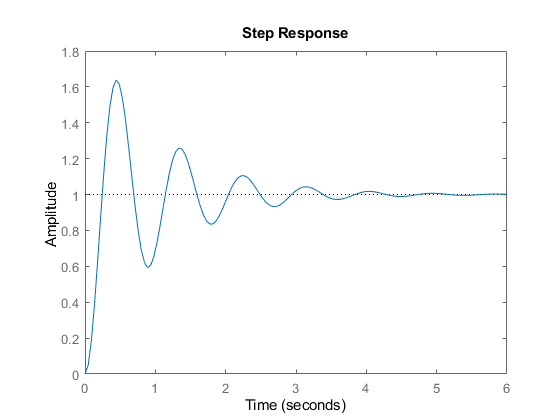
\includegraphics[width=\textwidth]{images/figure2.png}
    \end{subfigure}
\end{figure}

\begin{figure}[H]
    \centering
    \begin{subfigure}[b]{0.49\textwidth}
        \centering
        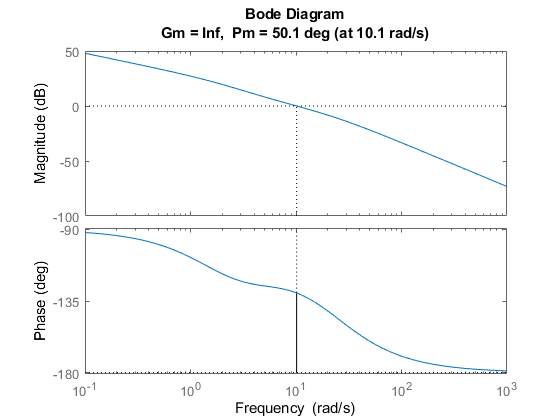
\includegraphics[width=\textwidth]{images/figure3.png}
    \end{subfigure}
    \hfill
    \begin{subfigure}[b]{0.49\textwidth}
        \centering
        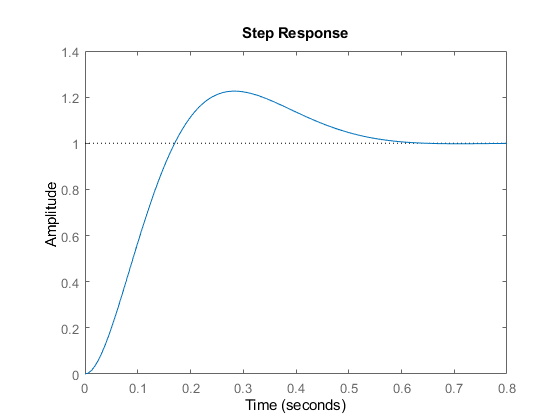
\includegraphics[width=\textwidth]{images/figure4.png}
    \end{subfigure}
\end{figure}

\begin{figure}[H]
    \centering 
 	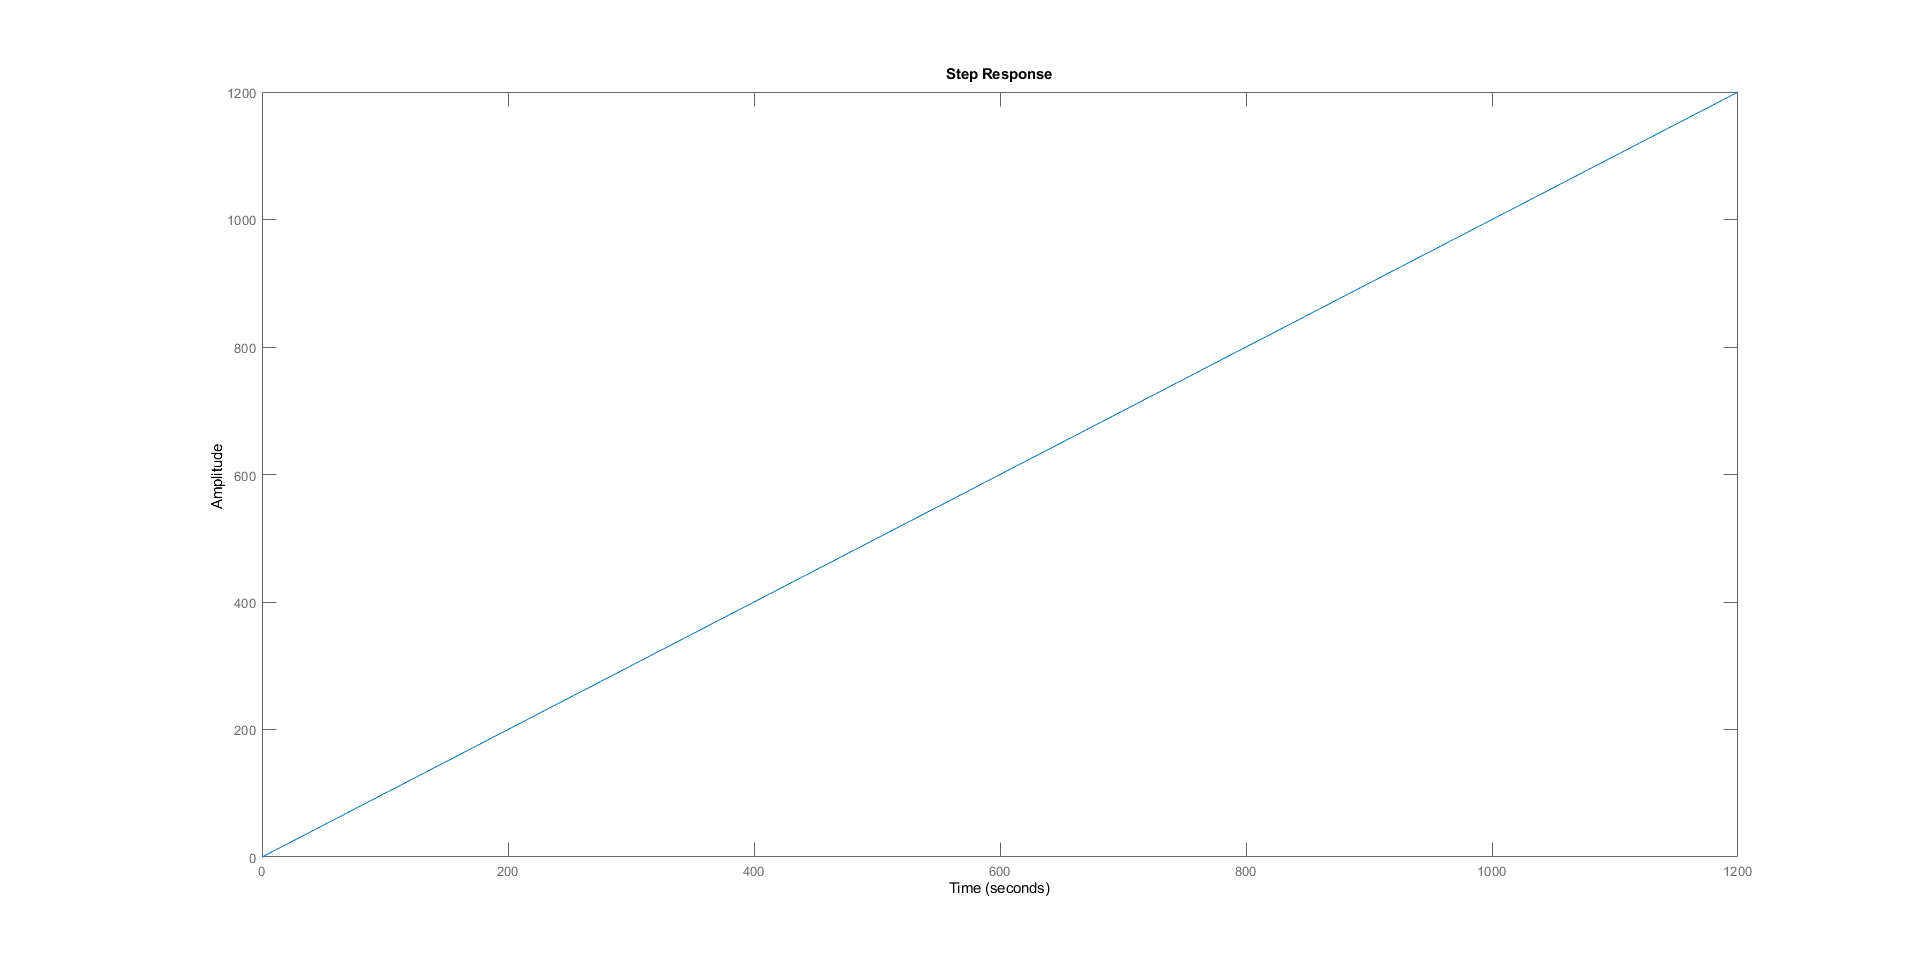
\includegraphics[width=\textwidth]{images/figure5.png}
\end{figure}

\begin{figure}[H]
    \centering 
 	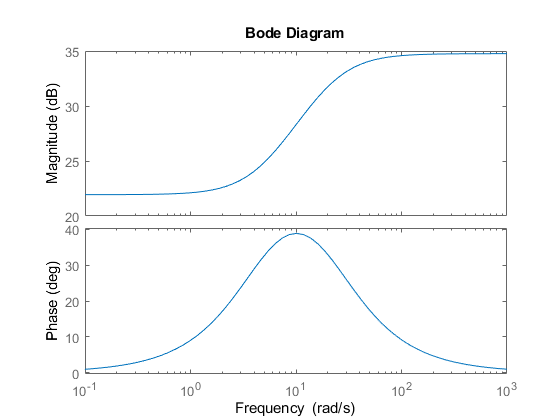
\includegraphics[width=\textwidth]{images/figure6.png}
\end{figure}

\noindent O código pode ser encontrado em meu github:

\href{https://github.com/slemanz/CONTROL_SYSTEM/blob/main/MATLAB/LEAD_COMPENSATOR/Gain_Kc.m}{\bfseries \color{BlueViolet} www.github.com/slemanz/CONTROL\textunderscore SYSTEM}








\end{document}
